\documentclass[11pt, spanish]{article}
\usepackage[utf8]{inputenc}
\usepackage{listings} 
\usepackage{graphicx}
\usepackage{color,soul}
\usepackage[dvipsnames]{xcolor}
\usepackage[T1]{fontenc}
\usepackage{bigfoot}
\usepackage{amsmath}
\usepackage{commath}
\usepackage[numbered,framed]{matlab-prettifier}
\usepackage{caption}
\usepackage[figurename=Figura, tablename=Tabla, font={small,tt}]{caption}

\makeatletter
    \setlength\@fptop{0\p@}
\makeatother

\usepackage{geometry}
 \geometry{
 a4paper,
 left=30mm,
 right=30mm,
 top=30mm,
 }

\date{}

\lstset{
	style              = Matlab-editor,
  	basicstyle         = \mlttfamily,
  	escapechar         = ",
  	mlshowsectionrules = true,
	framesep=4.5mm,
	framexleftmargin=2.5mm,
	fillcolor=\color{White},
	rulecolor=\color{Black},
	numberstyle=\normalfont\tiny\color{Black}
}

\captionsetup[lstlisting]{font={small,tt}}
\renewcommand{\lstlistingname}{Script}



\begin{document}

\renewcommand\lstlistlistingname{Lista de Scripts}

\author{Sebastián Valencia Calderón \\ 201111578}
\title{Laboratorio 1: Sistema numérico de punto flotante}
\maketitle

%====================================================================
\section{Introducción}

La aritmética de punto flotante, proporciona las bases para la representación de cantidades reales en un computador digital. Dado que los cálculos numéricos son de fundamental importancia para el diseño de sistemas de ingeniería, y solución de grandes y complejos sistemas matemáticos, conviene entender los modos de representación de una cantidad real en un computador, y las implicaciones que esto tiene para los cálculos en cuestión. Las implicaciones, radican en la limitación básica del sistema; un computador digital, permite únicamente la representación de cierto conjunto de números con precisión finita. Esta limitación física para la representación de las cantidades, puede traer errores en los cálculos numéricos ejecutados por algoritmos implementados sobre un lenguaje de programación.\\

En este caso en particular, se estudia tal representación y sus limitaciones haciendo uso de \textsc{MATLAB}, una poderosa herramienta de computación científica, en la cual resulta pertinente la implementación de algoritmos numéricos, por su facilidad para representar y manipular arreglos de números. Mediante distintas aproximaciones, se pretende conocer las limitaciones de representación de la maquina o mejor, la arquitectura de la maquina sobre los números reales. A través de las implementaciones realizadas, se pretende cumplir con los siguientes objetivos:

\begin{itemize}
\item Entender las características, ventajas y desventajas asociadas con las unidades de punto flotante que permiten el desarrollo de la computación numérica.

\item Observar casos que ilustran las precauciones que deben ser tenidas en cuenta en sistemas intensivos en computación numérica.
\end{itemize}


%==================================================================
\section{Procedimiento}

Para cumplir los objetivos enumerados anteriormente, se desarrollan algoritmos para encontrar el epsilon ($\epsilon_M$) de la maquina de un número particular. Con base en esto, se comparan los algoritmos, y de manera análoga, los resultados para un rango grande de los números representados en la máquina donde los algoritmos fueron ejecutados. Después, se procede con la experimentación sobre el rango de números representables, y las cantidades matemáticas fundamentales en \textsc{MATLAB}, posteriormente, se estudian y desarrollan algoritmos numéricos que manipulan la representación de los números para obtener las representaciones numéricas de los resultados ya conocidos de manera analítica.

De manera más desglosada, la ejecución de este laboratorio, procede de la siguiente forma:

\begin{enumerate}

\item Implementar un algoritmo numérico que halle de manera eficiente y certera el epsilon de la maquina ($\epsilon_M$), esto es el valor que caracteriza el nivel de precisión de una máquina. El epsilon de la máquina, es el número de punto flotante más pequeño tal que: \cite{forsythe1977computer}

$$1 + \epsilon_M > 1$$

La definición dada anteriormente, es caracterizada únicamente por un número representado en punto flotante. Luego de esto, se pretende generalizar el epsilon sobre cualquier número, es decir, para un número $x$, $\epsilon(x) = \epsilon \ ;\ \abs{x + \epsilon} > x$. Con una distribución representativa de los números en punto flotante representables por la máquina de trabajo, se pretende comparar distintos algoritmos para su cálculo, y su valor en términos de $x$.

\item Con base en el estándar IEEE 754-2008 \cite{ieeestd}, se estudia la representación y de constantes matemáticas de importancia analítica, es decir, la representación numérica de algunos resultados analíticos fundamentales. De la misma manera, se calcula el valor de funciones matemáticas de interés y conocimiento general, esto, con el fin de dilucidar las implicaciones que pueda tener el desarrollo de modelos con base en cálculos numéricos sobre un computador digital.

\end{enumerate}

%==================================================================
\section{Resultados}

A continuación, se evidencian los resultados y la metodología y herramientas de ejecución para cada uno de los problemas propuestos en la guía de laboratorio.

\begin{enumerate}

\item "El valor epsilon de una maquina es la diferencia entre 1.0 y el numero de punto flotante siguiente. Ya que este espaciamiento no es uniforme en todo el rango de representación de números de punto flotante, esta definición puede ser extendida alrededor de cualquier otro numero (diferente de 1.0) y escrita como $\epsilon_M(x)$ para cualquier numero de punto flotante $x$. Esta es una de las razones para calcular el valor de epsilon en \textsc{MATLAB} (el cual cuenta por defecto con un valor constante “eps”), adicionalmente, es conveniente conocer algunos algoritmos para computar este valor, ya que algunos lenguajes de programación no cuentan un valor predefinido del mismo." (Tomado de la guía de laboratorio).\\

En el script \ref{lst:MaqEpsOne}, se evidencia el diseño y escritura de un algoritmo para calcular $\epsilon_M$. El script, muestra el algoritmo propuesto en el enunciado. Después de su ejecución, el valor fue:

$$\epsilon_M = 2.220446049250313 \times 10 ^{-16}$$

La constante eps de \textsc{MATLAB}, es: $2..220446049250313 \times 10^{-16}$.

\item Para generalizar la definición de $\epsilon_M$, sobre cualquier número, se introduce el concepto de $\epsilon_M(x)$, es decir, el número en punto flotante más pequeño para el cual resulta que sumarlo a $x$, se tiene un número mayo a $x$ en la representación del computador. Es decir, $\epsilon(x) = \epsilon \ ;\ \abs{x + \epsilon} > x$. Para diseñar un algoritmo que compute esto, resulta pertinente recurrir al script \ref{lst:MaqEpsOne}, en este, se cuenta con un valor de inicializacion de $\epsilon$, de manera que $1.0 + epsilon > 1.0$. Para la generalización requerida, se debe tener un $\epsilon$, tal que $x + \epsilon > x$, de manera que se doble el valor de $\epsilon$, y se incremente la suma $x + \epsilon$ hasta que $x + \epsilon \leq x$, se ha encontrado el valor $2 \times \epsilon$. En el script \ref{lst:MaqEps}, se evidencia el desarrollo de un algortimo, que análogamente al enunciado anteriormente, reduce el valor de $\epsilon$, hasta que $x + \epsilon \leq x$.

\lstinputlisting[caption = {Gráfica de $x$ vs $\epsilon(x)$}, label={lst:plotEpsilon}]{data/scripts/plotEpsilon.m}

\begin{figure}[htbp]
\centering
	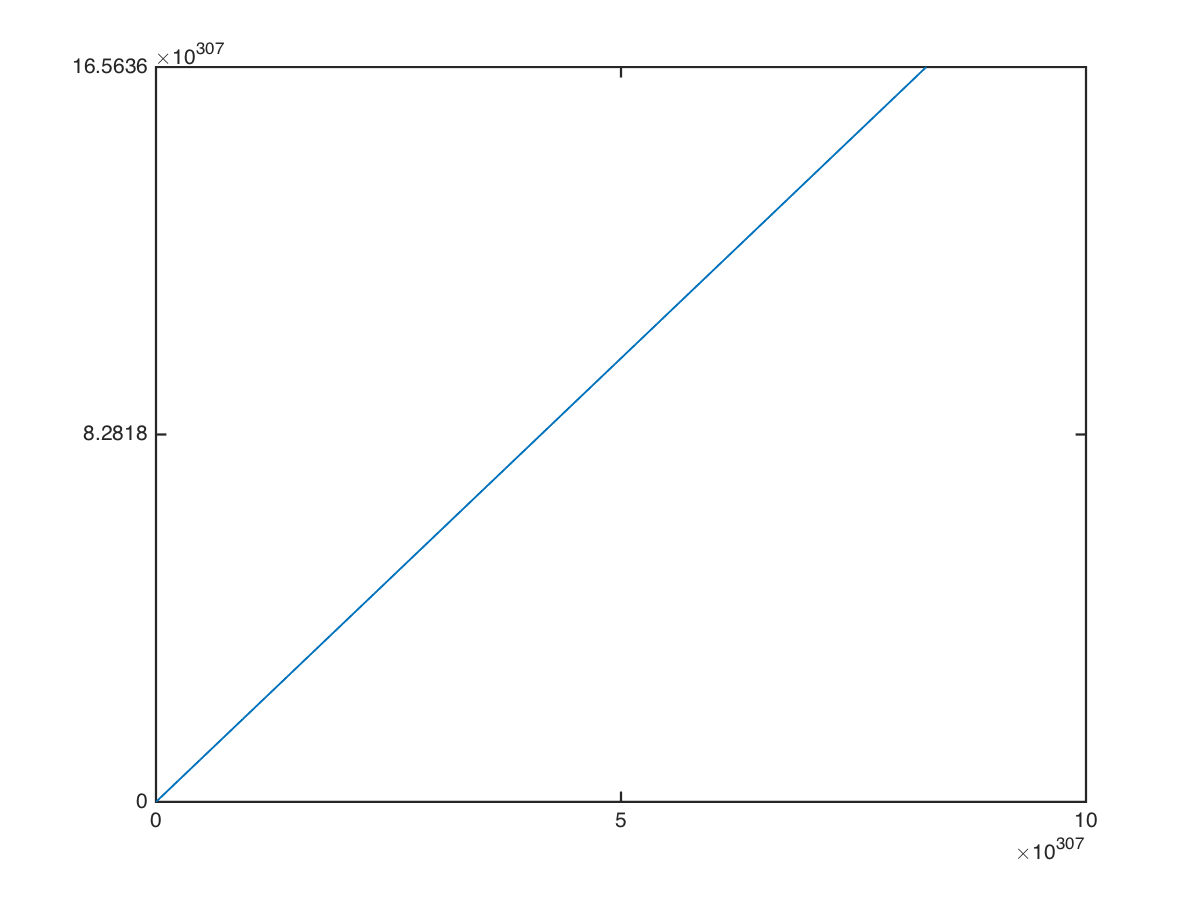
\includegraphics[scale=0.6]{data/img/plot_epsilon}
	\caption{Un ejemplo}
\end{figure}

\hl{ANALISIS DE LA GRAFICA}

\item El procedimiento diseñado por William Kahan, y utilizado en el paquete \textsc{LINPACK}, implementado en \textsc{FORTRAN 77} \cite{dongarra1979linpack}, tiene como objetivo estimar las unidades de redondeo en una cantidad proporcional al tamaño de $x$. Es decir, el epsilon para un $x$ en punto flotante. Sin embargo, asume ciertas características, que son riesgosas si no se usa este de manera adecuada. Por ejemplo, la base usada para la representación en punto flotante no debe ser potencia de tres. El código original, puede verse en el script \ref{lst:kahanFortran}.\\

Para analizar el desempeño de este y comparar sus resultados con los implementados previamente, se procede a implementar el algoritmo en \textsc{MATLAB}, realizar pequeños experimentos para comparar los valores, y posteriormente, realizar la prueba sobre un rango representativo de los números de punto flotante capaces de ser representados por la máquina digital que corre los programas.
\end{enumerate}

%==================================================================
\section{Conclusiones}

Lorem Ipsum is simply dummy text of the printing and typesetting industry. Lorem Ipsum has been the industry's standard dummy text ever since the 1500s, when an unknown printer took a galley of type and scrambled it to make a type specimen book. It has survived not only five centuries, but also the leap into electronic typesetting, remaining essentially unchanged. It was popularised in the 1960s with the release of Letraset sheets containing Lorem Ipsum passages, and more recently with desktop publishing software like Aldus PageMaker including versions of Lorem Ipsum.



\begin{itemize}
  \item Lorem Ipsum is simply dummy text of the printing and typesetting industry. Lorem Ipsum has been the industry's standard dummy text ever since the 1500s, when an unknown printer took a galley of type and scrambled it to make a type specimen book. It has survived not only five centuries, but also the leap into electronic typesetting, remaining essentially unchanged. It was popularised in the 1960s with the release of Letraset sheets containing Lorem Ipsum passages, and more recently with desktop publishing software like Aldus PageMaker including versions of Lorem Ipsum.
  
   \item Lorem Ipsum is simply dummy text of the printing and typesetting industry. Lorem Ipsum has been the industry's standard dummy text ever since the 1500s, when an unknown printer took a galley of type and scrambled it to make a type specimen book. It has survived not only five centuries, but also the leap into electronic typesetting, remaining essentially unchanged. It was popularised in the 1960s with the release of Letraset sheets containing Lorem Ipsum passages, and more recently with desktop publishing software like Aldus PageMaker including versions of Lorem Ipsum. \cite{norman}.
\end{itemize}

%==================================================================
\newpage
\section{Bibliografía}

\begingroup
\renewcommand{\section}[2]{}%
\begin{thebibliography}{}

  \bibitem{forsythe1977computer} Forsythe, G.E. and Malcolm, M.A. and Moler, C.B. {\em Computer methods for mathematical computations}, Prentice-Hall series in automatic computation. 1977.
  
  \bibitem{ieeestd} IEEE Task P754. {\em IEEE 754-2008, Standard for Floating-Point Arithmetic}, pub-IEEE-STD. 2008.
  
  \bibitem{dongarra1979linpack} Dongarra, J.J. and Bunch, J.R. and Moler, C.B. and Stewart, G.W. {\em LINPACK Users' Guide}, Society for Industrial and Applied Mathematics. 1979.
  
\end{thebibliography}
\endgroup

%==================================================================
\newpage
\section{Scripts}

\lstinputlisting[caption = {Cálculo de $\epsilon_M$}, label={lst:MaqEpsOne}]{data/scripts/MaqEpsOne.m}

\lstinputlisting[caption = {Cálculo de $\epsilon_M$ para un $x$ específico}, label={lst:MaqEps}]{data/scripts/MaqEps.m}

\lstinputlisting[caption = {Cálculo de $\epsilon_M(x)$ según el algoritmo de Kahan implementado en \textsc{FORTRAN}}, label={lst:kahanFortran}, language=Fortran]{data/scripts/kahan.f}

\addcontentsline{toc}{chapter}{\lstlistlistingname}
\lstlistoflistings

\bibliography{sample}

\end{document}
